\documentclass[tikz,border=2pt,11pt]{standalone}
\usetikzlibrary{positioning}
\usetikzlibrary{arrows.meta}
\usetikzlibrary{calc}
\usetikzlibrary{fit}
\usetikzlibrary{backgrounds}
\usepackage{amsmath}
\usepackage{amssymb}
\usepackage{xcolor}
\usepackage{graphicx}
\usepackage{tikz}
\newcommand{\R}{\mathbb{R}}
\newcommand{\C}{\mathbb{C}}
\newcommand{\N}{\mathbb{N}}
\newcommand{\Z}{\mathbb{Z}}
\DeclareMathOperator{\Ric}{Ric}
\DeclareMathOperator{\Rm}{Rm}
\DeclareMathOperator{\Scal}{Scal}
\DeclareMathOperator{\Vol}{Vol}
\DeclareMathOperator{\diam}{diam}
\DeclareMathOperator{\dist}{dist}
\DeclareMathOperator{\supp}{supp}
\DeclareMathOperator{\tr}{tr}
\DeclareMathOperator{\Id}{Id}
\DeclareMathOperator{\rank}{rank}
\begin{document}
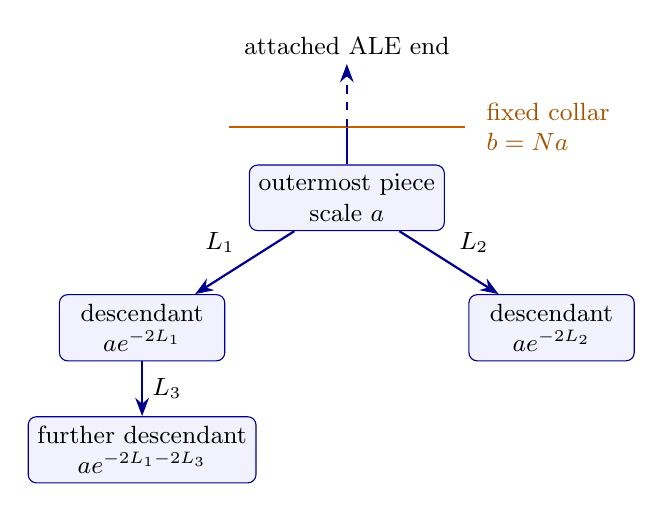
\begin{tikzpicture}[
  x=1cm,y=1cm,>=Stealth,
  piece/.style={draw=blue!55!black,fill=blue!5,rounded corners=3pt,
                minimum width=2.1cm,minimum height=.65cm,align=center},
  edge/.style={draw=blue!55!black,thick},
  every node/.style={font=\small}]
  \node[piece] (root) at (0,0) {outermost piece\\scale $a$};
  \node[piece] (left) at (-2.6,-1.65) {descendant\\$a e^{-2L_1}$};
  \node[piece] (right) at (2.6,-1.65) {descendant\\$a e^{-2L_2}$};
  \node[piece] (deep) at (-2.6,-3.2)
    {further descendant\\$a e^{-2L_1-2L_3}$};
  \draw[edge,->] (root) -- node[above left] {$L_1$} (left);
  \draw[edge,->] (root) -- node[above right] {$L_2$} (right);
  \draw[edge,->] (left) -- node[right] {$L_3$} (deep);
  \draw[edge] (root.north) -- (0,.9);
  \draw[draw=orange!75!black,thick] (-1.5,.9)--(1.5,.9);
  \node[right,align=left,text=orange!65!black] at (1.65,.9)
    {fixed collar\\$b=Na$};
  \draw[edge,dashed,->] (0,.9)--(0,1.7);
  \node[above] at (0,1.7) {attached ALE end};
\end{tikzpicture}
\end{document}
